\documentclass{article}
\usepackage{tikz}
\usetikzlibrary{trees}

\begin{document}

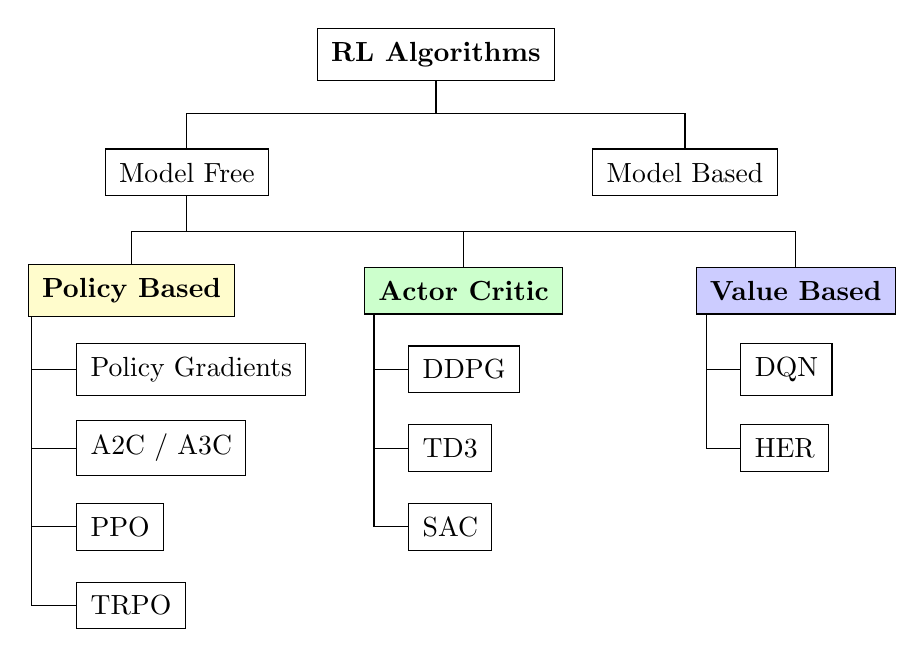
\begin{tikzpicture}[
		every node/.style={draw,inner sep=5pt},
		bold/.style={font=\bfseries},
		grandchild/.style={xshift=-2em,anchor=west,
			edge from parent path={(\tikzparentnode.195) |- (\tikzchildnode.180)}},
		level 1/.style={sibling distance=18em},
		level 2/.style={sibling distance=12em},
	]
	\coordinate
	node[bold] {RL Algorithms}
	[edge from parent fork down]
	child{
		node {Model Free}
		child[xshift=10em] {
			node[bold,fill=yellow!20] {Policy Based}
			[grow via three points={one child at (0,-1) 
				and two children at (0,-1) and (0,-2)}]
			child[grandchild] {node {Policy Gradients}}
			child[grandchild] {node {A2C / A3C}}
			child[grandchild] {node {PPO}}
			child[grandchild] {node {TRPO}}
		}
		child[xshift=10em] {
			node[bold,fill=green!20] {Actor Critic}
			[grow via three points={one child at (0,-1) 
				and two children at (0,-1) and (0,-2)}]
			child[grandchild] {node {DDPG}}
			child[grandchild] {node {TD3}}
			child[grandchild] {node {SAC}}
		}
		child[xshift=10em] {
			node[bold,fill=blue!20] {Value Based}
			[grow via three points={one child at (0,-1) 
				and two children at (0,-1) and (0,-2)}]
			child[grandchild] {node {DQN}}
			child[grandchild] {node {HER}}
		}
	}
	child{
		node {Model Based}
	};
\end{tikzpicture}

\end{document}
